%%%%%%%%%%%%%%%%%%%%%%%%%%%%%%%%%%%%%%%%%
% Short Sectioned Assignment LaTeX Template Version 1.0 (5/5/12)
% This template has been downloaded from: http://www.LaTeXTemplates.com
% Original author:  Frits Wenneker (http://www.howtotex.com)
% License: CC BY-NC-SA 3.0 (http://creativecommons.org/licenses/by-nc-sa/3.0/)
%%%%%%%%%%%%%%%%%%%%%%%%%%%%%%%%%%%%%%%%%

%----------------------------------------------------------------------------------------
%	PACKAGES AND OTHER DOCUMENT CONFIGURATIONS
%----------------------------------------------------------------------------------------

\documentclass[paper=a4, fontsize=11pt]{scrartcl} % A4 paper and 11pt font size

% ---- Entrada y salida de texto -----

\usepackage[T1]{fontenc} % Use 8-bit encoding that has 256 glyphs
\usepackage[utf8]{inputenc}
%\usepackage{fourier} % Use the Adobe Utopia font for the document - comment this line to return to the LaTeX default

% ---- Idioma --------

\usepackage[spanish, es-tabla]{babel} % Selecciona el español para palabras introducidas automáticamente, p.ej. "septiembre" en la fecha y especifica que se use la palabra Tabla en vez de Cuadro

% ---- Otros paquetes ----

\usepackage{url} % ,href} %para incluir URLs e hipervínculos dentro del texto (aunque hay que instalar href)
\usepackage{amsmath,amsfonts,amsthm} % Math packages
%\usepackage{graphics,graphicx, floatrow} %para incluir imágenes y notas en las imágenes
\usepackage{graphics,graphicx, float} %para incluir imágenes y colocarlas

% Para hacer tablas comlejas
%\usepackage{multirow}
%\usepackage{threeparttable}

%\usepackage{sectsty} % Allows customizing section commands
%\allsectionsfont{\centering \normalfont\scshape} % Make all sections centered, the default font and small caps

\usepackage{fancyhdr} % Custom headers and footers
\pagestyle{fancyplain} % Makes all pages in the document conform to the custom headers and footers
\fancyhead{} % No page header - if you want one, create it in the same way as the footers below
\fancyfoot[L]{} % Empty left footer
\fancyfoot[C]{} % Empty center footer
\fancyfoot[R]{\thepage} % Page numbering for right footer
\renewcommand{\headrulewidth}{0pt} % Remove header underlines
\renewcommand{\footrulewidth}{0pt} % Remove footer underlines
\setlength{\headheight}{13.6pt} % Customize the height of the header

\numberwithin{equation}{section} % Number equations within sections (i.e. 1.1, 1.2, 2.1, 2.2 instead of 1, 2, 3, 4)
\numberwithin{figure}{section} % Number figures within sections (i.e. 1.1, 1.2, 2.1, 2.2 instead of 1, 2, 3, 4)
\numberwithin{table}{section} % Number tables within sections (i.e. 1.1, 1.2, 2.1, 2.2 instead of 1, 2, 3, 4)

\setlength\parindent{0pt} % Removes all indentation from paragraphs - comment this line for an assignment with lots of text

\newcommand{\horrule}[1]{\rule{\linewidth}{#1}} % Create horizontal rule command with 1 argument of height

\graphicspath{ {./images/} }
\usepackage{subcaption}
\usepackage{hyperref}
\usepackage{soul}

%----------------------------------------------------------------------------------------
%	TÍTULO Y DATOS DEL ALUMNO
%----------------------------------------------------------------------------------------

\title{	
\normalfont \normalsize 
\textsc{\textbf{Recuperación de Información (2018-2019)} \\ Doble Grado en Ingeniería Informática y Matemáticas \\ Universidad de Granada} \\ [25pt] % Your university, school and/or department name(s)
\horrule{0.5pt} \\[0.4cm] % Thin top horizontal rule
\huge Memoria Práctica 3: \\Implementación de un Sistema de
Recuperación de Información utilizando
Lucene \\ % The assignment title
\horrule{2pt} \\[0.5cm] % Thick bottom horizontal rule
}

\author{Luis Balderas Ruiz \\ \texttt{luisbalderas@correo.ugr.es}} 
 % Nombre y apellidos 


\date{\normalsize\today} % Incluye la fecha actual

%----------------------------------------------------------------------------------------
% DOCUMENTO
%----------------------------------------------------------------------------------------

\begin{document}

\maketitle % Muestra el Título

\newpage %inserta un salto de página

\tableofcontents % para generar el índice de contenidos

\newpage

\section{Introducción}

El objetivo de esta práctica es diseñar un Sistema de Recuperación de Información utilizando la biblioteca Lucene. Más concretamente, crearé un buscador sobre un conjunto de preguntas y respuestas sobre el lenguaje de programación R. En total, podemos encontrar más de 85000 preguntas y 82000 respuestas que conformarán nuestra base de datos documental. Dicho sistema estará dividido en dos subsistemas que tendrán las siguientes funciones:

\begin{itemize}
	\item El primer subsistema será el encargado de recibir, procesar los datos y crear el índice.
	\item El segundo, ideado para ser utilizado por el usuario, será una aplicación de escritorio sobre la que se pueda hacer consultas y mostrará los documentos relevantes
\end{itemize}


En el presente documento se expondrá el análisis de requisitos de ambos subsistemas y un manual de usuario para su uso. 

\section{Análisis de Requisitos}

\subsection{Subsistemas}

Como acabo de comentar, dividiré el sistema en dos subsistemas de información independientes: Subsistema Central y RQuerySystem. A continuación, se describe la funcionalidad de cada uno de ellos.

\subsubsection{Subsistema central}

El subsistema central será únicamente utilizado por el administrador del sistema principal. Su cometido es recibir los datos y procesarlos según los criterios estudiados en las prácticas anteriores, de forma que se encuentren en perfectas condiciones para ser indexados y consultados posteriormente. 

\subsubsection{RQuerySystem}

Encarna la aplicación principal de sistema. Generado previamente el índice, permitirá consultas por parte de los usuarios y responderá a sus peticiones con los documentos más relevantes mediante una interfaz gráfica muy intuitiva. En ella se puede buscar por facetas y hacer consultas relativamente complejas en varios campos con operadores lógicos.

\begin{figure}[H] %con el [H] le obligamos a situar aquí la figura
	\centering
	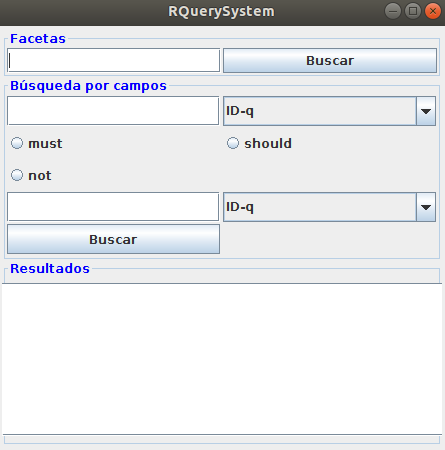
\includegraphics[scale=0.5]{resultado.png}  %el parámetro scale permite agrandar o achicar la imagen. En el nombre de archivo puede especificar directorios
	\caption{Imagen de la interfaz gráfica de la app} 
\end{figure}


\subsection{Requisitos funcionales}

Expongo los distintos requisitos funcionales y los relaciono con los requisitos de datos.

\subsubsection{Requisitos funcionales del subsistema central}

\begin{itemize}
	\item \textbf{RF 1:} Recibir los datos en formato CSV. Datos de entrada: RD 1.1.
	\item \textbf{RF 2:} Procesar los datos utilizando distintos Analyzers de Lucene dependiendo del campo. Datos de entrada: RD 1.2. Datos de salida: RD 1.3.
	\item \textbf{RF 3:} Crear el índice. Datos de entrada: RD 1.4.
\end{itemize}

\subsubsection{Requisitos funcionales de RQuerySystem}

\begin{itemize}
	\item \textbf{RF 1:} Recibir y procesar consultas de un usuario. Datos de entrada: RD 2.1
	\item \textbf{RF 2:} Hacer búsqueda en el índice sobre los datos recibidos. Datos de entrada: RD 2.2. Salida: RD 2.3
	\item \textbf{RF 3:} Mostrar los documentos relevantes a la consulta. Datos de salida: RD 2.4.
\end{itemize}

\subsection{Requisitos de datos}

Expongo los distintos requisitos de datos.

\subsubsection{Requisitos de datos del subsistema central}

\begin{itemize}
	\item \textbf{RD 1.1:} Questions.csv, Answers.csv, Tags.csv
	\item \textbf{RD 1.2:} Mismos que en RD 1.1.
	\item \textbf{RD 1.3:} Datos de RD 1.2 modificados mediante Analyzers y tokenizados.
	\item \textbf{RD 1.4:} Mismos que en RD 1.4.
\end{itemize}

\subsubsection{Requisitos de datos de RQuerySystem}

\begin{itemize}
	\item \textbf{RD 2.1:} Texto en lenguaje natural (en inglés) y selección de la condición booleana entre consultas.
	\item \textbf{RD 2.2:} Mismos que en RD 2.1.
	\item \textbf{RD 2.3:} Resultados de la búsqueda en el índice.
	\item \textbf{RD 2.4:} Los mismos que en RD 2.3 presentados al usuario.
\end{itemize}

\subsubsection{Requisitos semánticos de RQuerySystem}
\begin{itemize}
	\item \textbf{RS 2.1} Se deben rellenar \textbf{todos} los campos que se expongan en la GUI.
\end{itemize}

\subsection{Esquemas}

\begin{figure}[H] %con el [H] le obligamos a situar aquí la figura
	\centering
	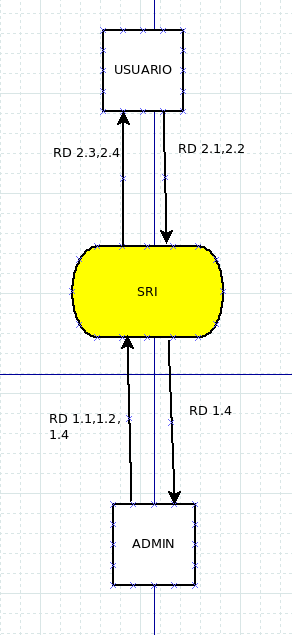
\includegraphics[scale=0.5]{caja-negra.png}  %el parámetro scale permite agrandar o achicar la imagen. En el nombre de archivo puede especificar directorios
	\caption{Esquema de caja negra del sistema} 
\end{figure}

\begin{figure}[H] %con el [H] le obligamos a situar aquí la figura
	\centering
	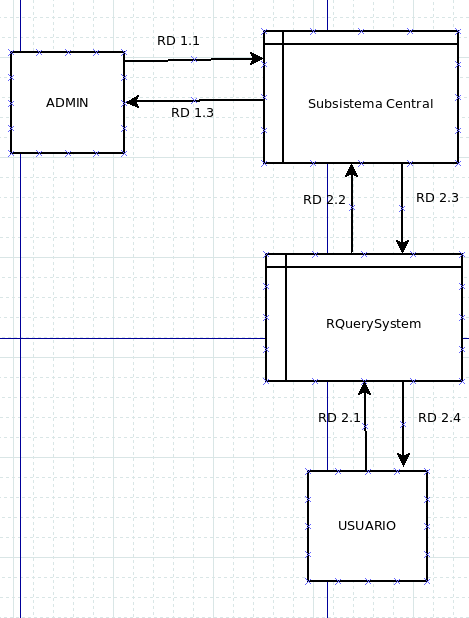
\includegraphics[scale=0.5]{armazon.png}  %el parámetro scale permite agrandar o achicar la imagen. En el nombre de archivo puede especificar directorios
	\caption{Esquema de f-armazón del sistema} 
\end{figure}

\begin{figure}[H] %con el [H] le obligamos a situar aquí la figura
	\centering
	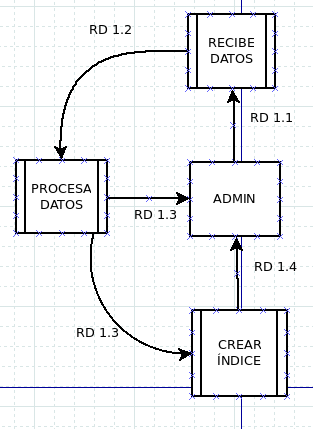
\includegraphics[scale=0.5]{c-fd.png}  %el parámetro scale permite agrandar o achicar la imagen. En el nombre de archivo puede especificar directorios
	\caption{Flujo de datos del subsistema central} 
\end{figure}

\begin{figure}[H] %con el [H] le obligamos a situar aquí la figura
	\centering
	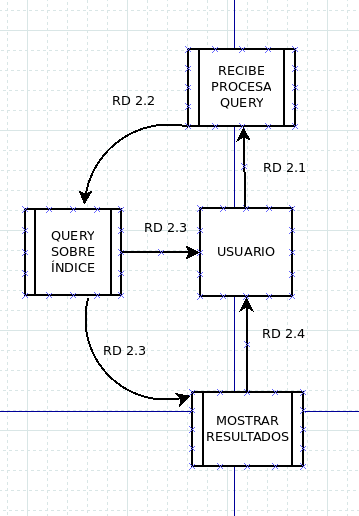
\includegraphics[scale=0.5]{r-fd.png}  %el parámetro scale permite agrandar o achicar la imagen. En el nombre de archivo puede especificar directorios
	\caption{Flujo de datos RQuerySystem (Mostrar datos representa a la interfaz de usuario)} 
\end{figure}

\subsubsection{Diagramas de clase}

\begin{figure}[H] %con el [H] le obligamos a situar aquí la figura
	\centering
	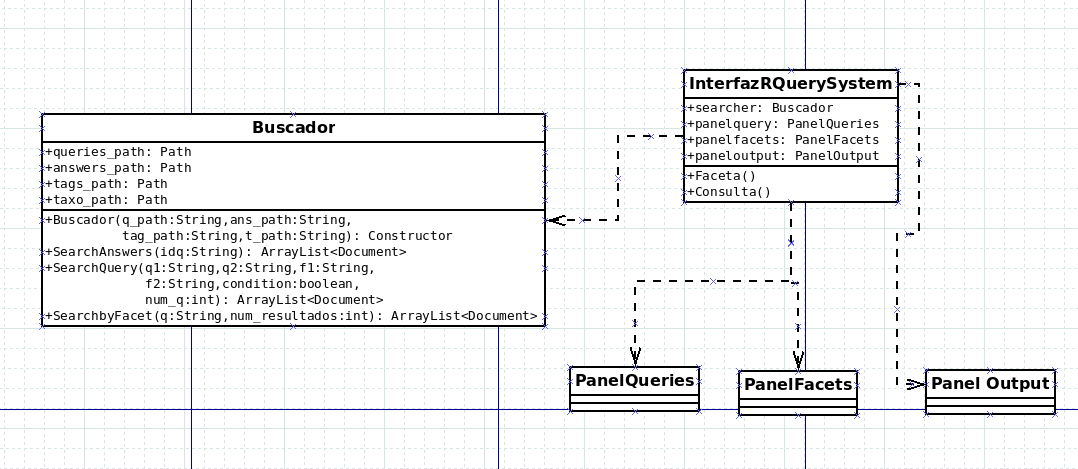
\includegraphics[scale=0.4]{dcrqs.png}  %el parámetro scale permite agrandar o achicar la imagen. En el nombre de archivo puede especificar directorios
	\caption{Diagrama de clases RQSystem} 
\end{figure}



\begin{figure}[H] %con el [H] le obligamos a situar aquí la figura
	\centering
	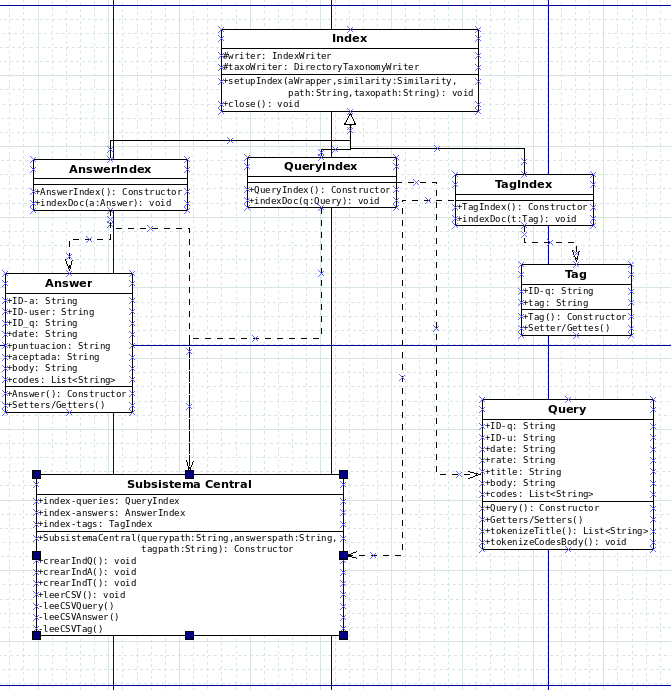
\includegraphics[scale=0.5]{dcsc.png}  %el parámetro scale permite agrandar o achicar la imagen. En el nombre de archivo puede especificar directorios
	\caption{Diagrama de clases Subsistema central} 
\end{figure}





\newpage
\section{Manual de usuario}

El diseño de este sistema está totalmente pensado para usuarios sin ninguna formación previa en consultas sobre índices. Con esta idea, utilizo un QueryParser en las consultas por campos, luego admite de manera total el lenguaje natural. El usuario podrá elegir en qué campo buscar cada consulta y cómo están relacionadas entre sí ambas. La primera siempre aparece y condiciona la disposición de la segunda. Los resultados se mostrarán en el cuadro de texto correspondiente. Por defecto, el número de salidas es 20, buscando 5 respuestas a cada pregunta formulada en el dataset. Con la intención de mejorar las inconsistencias que se dan a veces en los foros de StackOverFlow (las respuestas dadas por los usuarios pueden ser totalmente contradictorias), las respuestas que incluyo son aquellas que han sido aceptadas y las muestro ordenadas por la puntuación, no por el score que me devuelve la función similarity. Por tanto, la salida del programa devuelve un conjunto de preguntas almacenadas en el dataset ordenadas por BM25similarity y, asociada a cada pregunta, un conjunto de máximo 5 respuestas aceptadas (incluído como Facet para posibles modificaciones futuras, implementado como BooleanQuery) a dicha pregunta ordenadas por la puntuación recibida en la plataforma.
\\

Para el desarrollo de facetas o categorías he actuado a la manera de StackOverflow. Doy la posibilidad de buscar por categorías (almacenadas en el archivo Tag.csv). Esas categorías están asociadas a un \textit{ID-q} que luego busco sobre el índice de preguntas. Por supuesto, si se introduce un valor que no está contemplado como categoría, el resultado será vacío.
\\

Es un requisito para la utilización del programa que se rellenen todos los campos en uso, i.e., si se hace búsqueda por campos es necesario completar los dos cuadros de texto con su campo y decir qué relación hay entre ellos.

\end{document}